%%%%%%%%%%%%%%%%%%%%%%%%%%%%%%%%%%%%%%%%%%%%%%%%%%%%%%%%%%%%%%%%%%
%%%%%%%% ICML 2013 EXAMPLE LATEX SUBMISSION FILE %%%%%%%%%%%%%%%%%
%%%%%%%%%%%%%%%%%%%%%%%%%%%%%%%%%%%%%%%%%%%%%%%%%%%%%%%%%%%%%%%%%%

% Use the following line _only_ if you're still using LaTeX 2.09.
%\documentstyle[icml2013,epsf,natbib]{article}
% If you rely on Latex2e packages, like most moden people use this:
\documentclass{article}

% For figures
\usepackage{graphicx} % more modern
%\usepackage{epsfig} % less modern
% \usepackage{subfigure}
\usepackage{subcaption}
\usepackage{multicol}

% For citations
\usepackage{natbib}

% For algorithms
\usepackage{algorithm}
\usepackage{algorithmic}

% For math
\usepackage{amsmath}
\usepackage{siunitx}

% As of 2011, we use the hyperref package to produce hyperlinks in the
% resulting PDF.  If this breaks your system, please commend out the
% following usepackage line and replace \usepackage{icml2013} with
% \usepackage[nohyperref]{icml2013} above.
\usepackage{hyperref}

% Packages hyperref and algorithmic misbehave sometimes.  We can fix
% this with the following command.
\newcommand{\theHalgorithm}{\arabic{algorithm}}

% Employ the following version of the ``usepackage'' statement for
% submitting the draft version of the paper for review.  This will set
% the note in the first column to ``Under review.  Do not distribute.''
\usepackage{icml2013}
% Employ this version of the ``usepackage'' statement after the paper has
% been accepted, when creating the final version.  This will set the
% note in the first column to ``Proceedings of the...''
% \usepackage[accepted]{icml2013}


% The \icmltitle you define below is probably too long as a header.
% Therefore, a short form for the running title is supplied here:
\icmltitlerunning{6.867: Final Project}

\begin{document}

\twocolumn[
  \icmltitle{6.867: Final Project}

  % % It is OKAY to include author information, even for blind
  % % submissions: the style file will automatically remove it for you
  % % unless you've provided the [accepted] option to the icml2013
  % % package.
  % \icmlauthor{Andrea Li}{liandrea@mit.edu}
  % \icmladdress{Your Fantastic Institute,
  %             314159 Pi St., Palo Alto, CA 94306 USA}
  % \icmlauthor{Tyson Chen}{ytchen33@mit.edu}
  % \icmladdress{Their Fantastic Institute,
  %             27182 Exp St., Toronto, ON M6H 2T1 CANADA}

  % You may provide any keywords that you
  % find helpful for describing your paper; these are used to populate
  % the "keywords" metadata in the PDF but will not be shown in the document

  \vskip 0.3in
]

\section{Introduction}

\section{Data collection}
In order to collect season data, we primarily used publicly available data from \texttt{http://basketballvalue.com/downloads.php}.
Basic statistics, including points allowed and points scored, were available for seasons 2005-2011, and more sophisticated statistics, including rebounds, were avilable for seasons 2008-2011.

Many of the features generated for training and testing our classifier were derived from this game data. In order to create a general proxy for how strong a team was, we calculated running averages of points allowed, points scored, win rate, etc. and used these as input features to our classifier. These running averages were initialized to equal numbers for all teams at the beginning of the season and were subsequently updated as more data became available. Because these numbers were arbitrarily initialized to equal at the beginning of the season however, running averages near the beginning of the season serve as less reliable data points, as outliers can significantly affect the running average.

These statistics were therefore plotted over time throughout the season in order to approximate when the running averages for each of these statistics stabilized to reliable averages. Example plots are given in Figures 1 and 2, in which the running average win rate and points scored for a given team is plotted over course of the season.

\begin{figure}[width=\linewidth]
\centering
  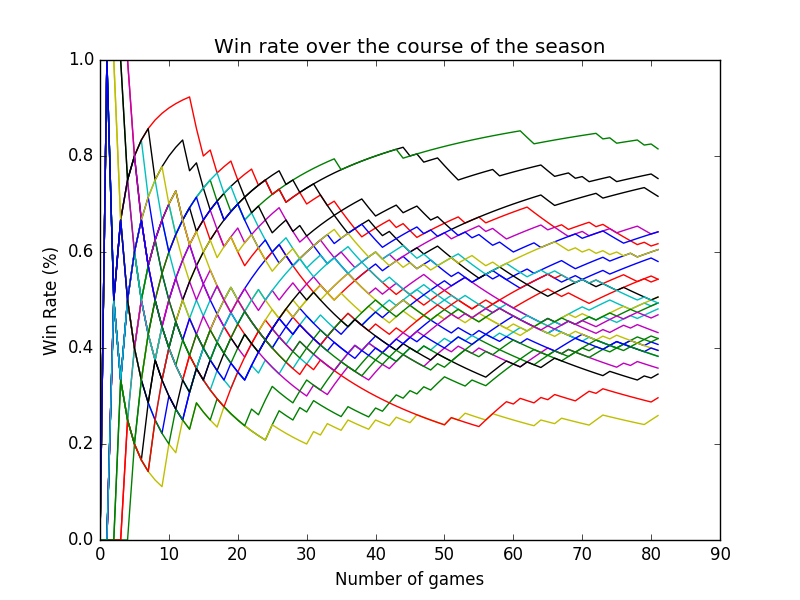
\includegraphics[width=1\linewidth]{code/figures/win_rate.png}
\caption{Win rate over time}
\end{figure}

\begin{figure}[width=\linewidth]
\centering
  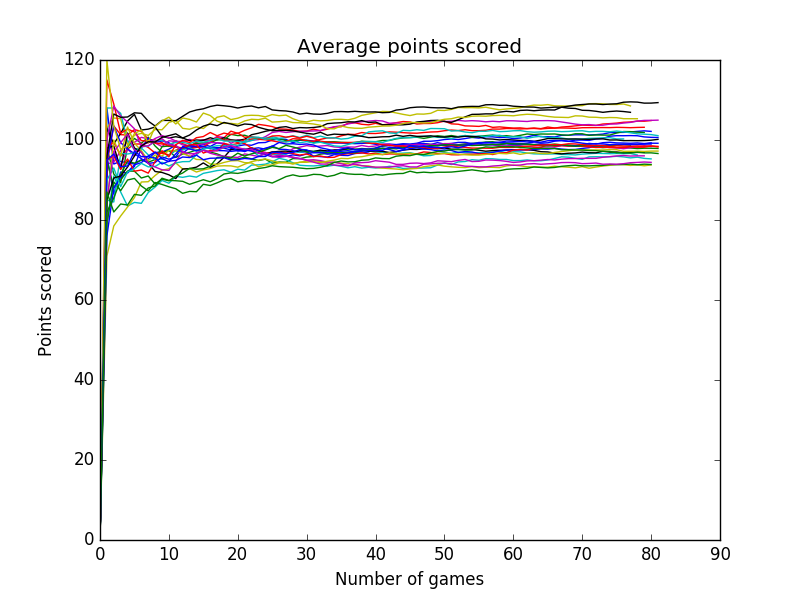
\includegraphics[width=1\linewidth]{code/figures/points_scored.png}
\caption{Points scored over time}
\end{figure}

In general, the running averages of the game data stabilized after approximately each team's twentieth game of the season. When generating our training, validation, and test sets therefore, we only used data after each team's twentieth game in order to ensure that the features extracted from the data were representative of true team performance.

In order to compare our algorithm and our predicted spreads against Vegas and other betting authorities, we created a scraper to scrape relevant websites with both current and historical spreads. We primarily scraped this information from \texttt{http://www.sportsbookreview.com/betting-odds/} \texttt{nba-basketball/}.

\section{Linear classifier}
As a baseline, we used our own implementation of a linear classifier on basic features including running averages of home/away team points scored, points allowed, Elo score, games won, games played, and win rate. Based on the 2006-2007 season, in predicting win/loss (as opposed to the spread of a win/loss), the linear classifier had an accuracy of 64.3\% on training data and 63.3\% on testing data.

After adding further features, such as home court advantage, were added to the model, the linear classifier has an accuracy of 72.3\% on training data and 66.9\% on testing data based on the 2008-2009 season.

We additionally explored the ability of the classifier to predict spreads on games, in which the margin of victory is taken into account instead of a simple win/loss. In this case, the accuracy metric was the absolute value of the difference between the predicted spread and the actual spread. Using basic features on the 2006-2007 season, the average absolute value spread error was 9.31 points for training data and 10.07 points for testing data.

After adding further features, the average absolute value spread error decreased to 8.53 points for training data but increased to 13.60 points for testing data. This would imply that the classifier might be overfitting to the features that are provided as input to the algorithm, which would be expected for more complex architectures but was surprising in the context of the linear classifier explored here.

These results for the performance of the linear classifier are summarized in Table 1.
\begin{table}
  \begin{center}
    \begin{tabular}{ | c | c | c | }
      \hline
                      & Win/Lose Accuracy & Spread Error  \\ \hline
      Basic features  & 63.3\%            & 10.07         \\ \hline
      Extra features  & 66.9\%            & 13.60         \\ \hline
    \end{tabular}
  \end{center}
  \caption{Classifier performance on test dataset}
\end{table}

Similar results were found when we used a polynomial basis and allowed the degree of the polynomial fitting the data to grow. Out of values for $M \in [1, 10]$, we found that a regression model with $M=1$ performed best, where $M=10$ on the other side of the spectrum led to extreme overfitting. The average spread error is summarized in Table 2 for each of the different possible values for $M$, and graphs for representative values of $M$ are illustrated in Figure 3. Note that for ease of illustration of data here, only the win rate feature is used as the feature vector

\begin{table}
  \begin{center}
    \begin{tabular}{ | c | c | c | c | c | }
      \hline
      \textbf{M=1}    & \textbf{M=2}    & \textbf{M=3}     & \textbf{M=4}     & \textbf{M=5}      \\ \hline
      10.15  & 11.35  & 11.013  & 12.40   & 11.32    \\ \hline
      \textbf{M=6}    & \textbf{M=7}    & \textbf{M=8}     & \textbf{M=9}     & \textbf{M=10}     \\ \hline
      12.05  & 33.26  & 33.56   & 17.11   & 150.23   \\ \hline
    \end{tabular}
  \end{center}
  \caption{Average spread error for M values}
\end{table}

\begin{figure}[width=\linewidth]
\centering
\begin{multicols}{2}
  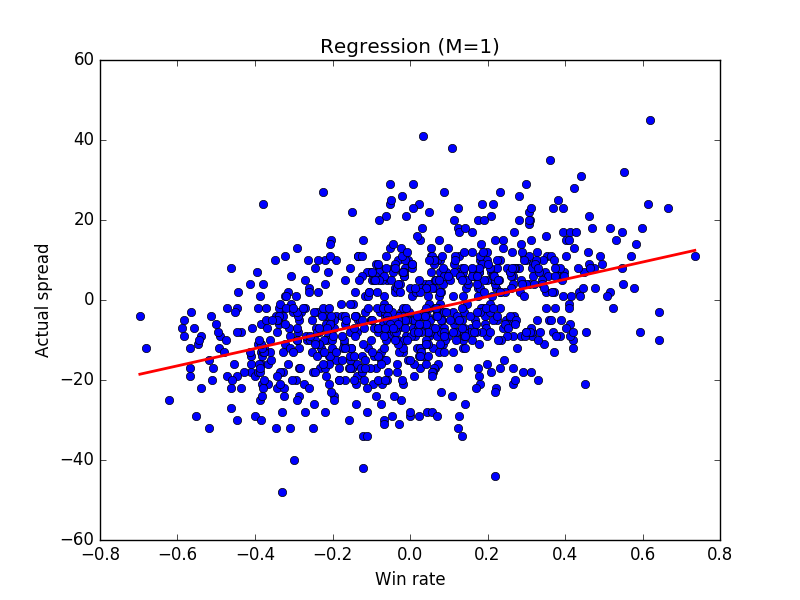
\includegraphics[width=1.2\linewidth]{code/figures/linear_regression(m=1).png}
  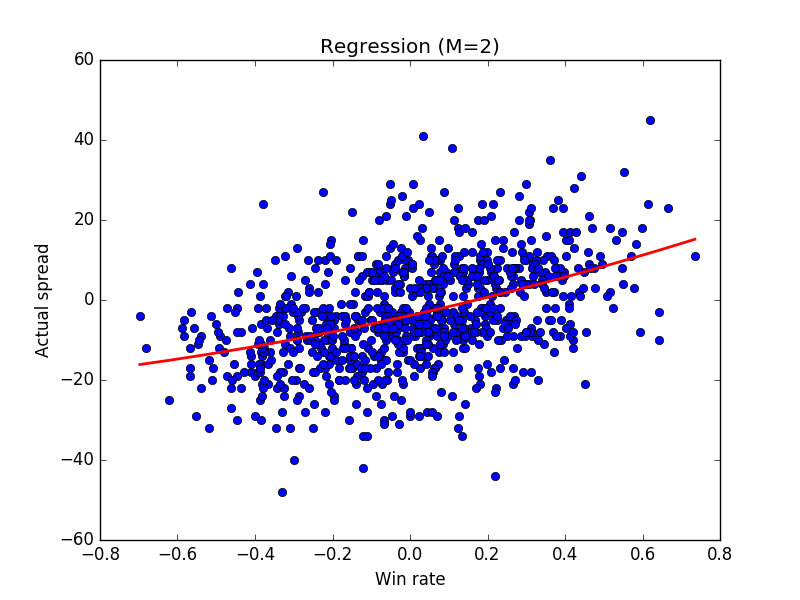
\includegraphics[width=1.2\linewidth]{code/figures/linear_regression(m=2).png}
  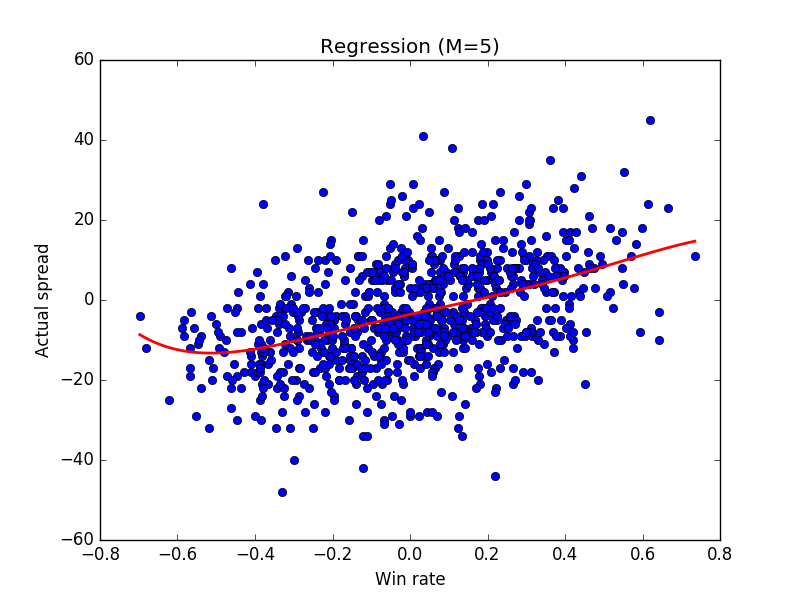
\includegraphics[width=1.2\linewidth]{code/figures/linear_regression(m=5).png}
  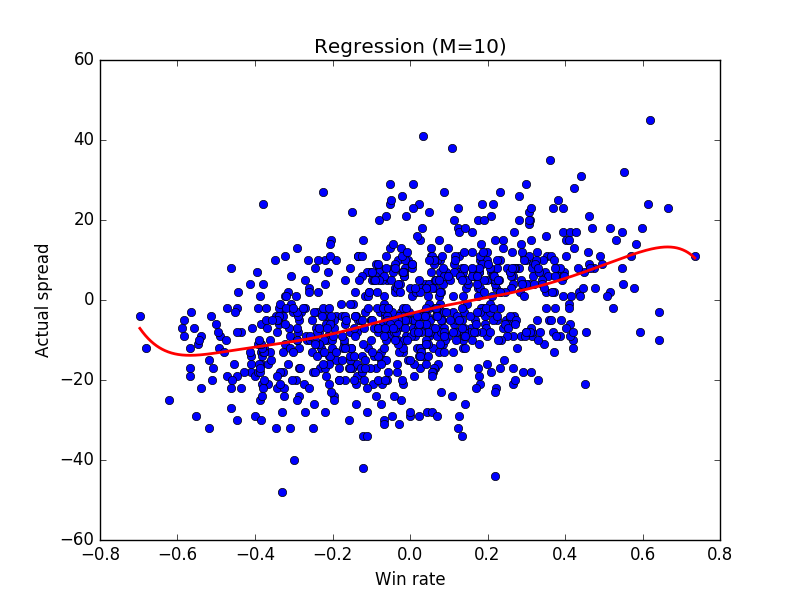
\includegraphics[width=1.2\linewidth]{code/figures/linear_regression(m=10).png}
\end{multicols}
\caption{Win rate vs. actual spread}
\end{figure}

We additionally explored the use of generating training, validation, and testing datasets across multiple seasons of data. In this case, because we train the model against certain features of the teams playing (e.g. running average win rate, average points scored, average points allowed, etc.), and not the skill level associated with the team itself, we can aggregate data across multiple seasons. This holds true even if teams and their respective players have changed significantly between seasons, because the features we draw from the data are running averages calculated from the season so far.

When we run the linear classifier on three seasons worth of data, in which the training, validation, and testing datasets are each made up of a season of data (about 1300 games), the accuracy of the algorithm improves as expected. More specifically, when run on three seasons of data, the linear classifier is able to classify win/loss of matchups with an accuracy of 72.3\% on training data and 68.6\% on testing data. In terms of spreads, the linear classifier predicts spreads with an average spread error of 8.98 points on training data and 9.29 points on testing data. Thus, increasing the size of the data set has a fairly significant improvement in the accuracy of the linear classifier when compared with the 66.9\% accuracy previously obtained for win/loss predictions and 13.60 spread error for spread predictions.

As previously mentioned, we explored classification of the linear classifier with a set of basic features and a set of more complex partially derived from these basic features. The basic features included each team's Elo score, average points scored, average points allowed, number of games played, number of games won, and win rate. The additional features we added included home court advantage (e.g. home court average points scored, home court average points allowed, home court win rate, etc.) as well as possessions, offensive rebounds, and defensive rebounds. In order to understand which features contributed most heavily to the win/loss and spreads predictions, we plotted the weights of each of the features. These relative weights are illustrated in Figure 4, in which the win rate features (away team win rate, home team win rate, away team home court win rate, and home team home court win rate) were in general the most important features. For three seasons of data however in win/loss predictions, the other features contributed much more relative to the classifiers for spreads predictions and one season of data.

\begin{figure}[width=\linewidth]
\centering
\begin{multicols}{2}
  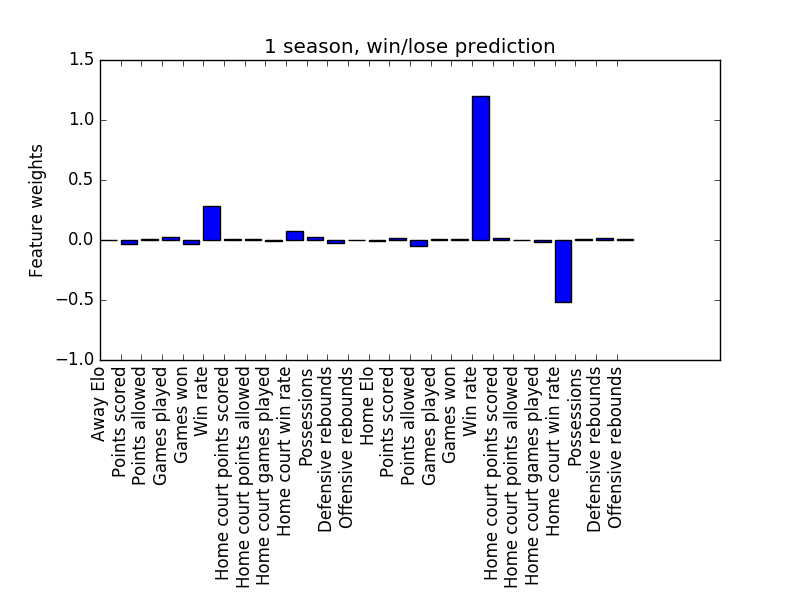
\includegraphics[width=1.2\linewidth]{code/figures/1season,winlose.png}
  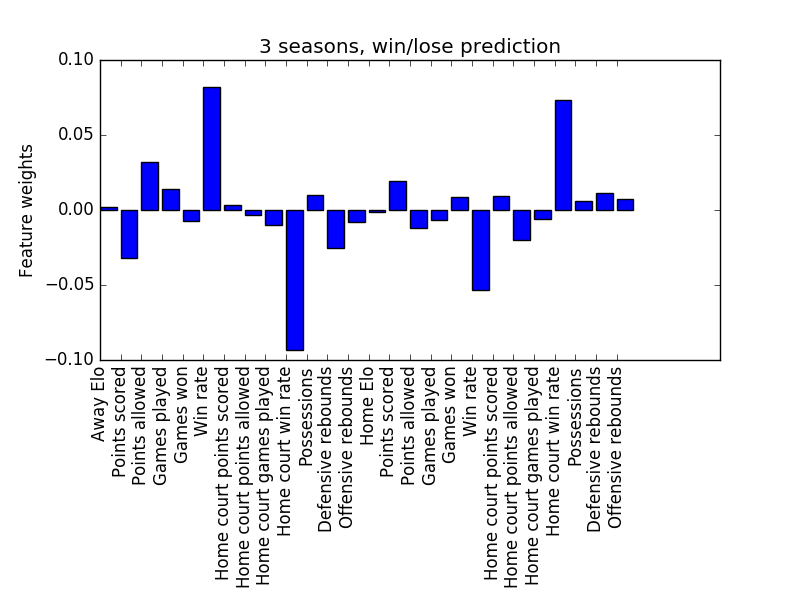
\includegraphics[width=1.2\linewidth]{code/figures/3seasons,winlose.png}
  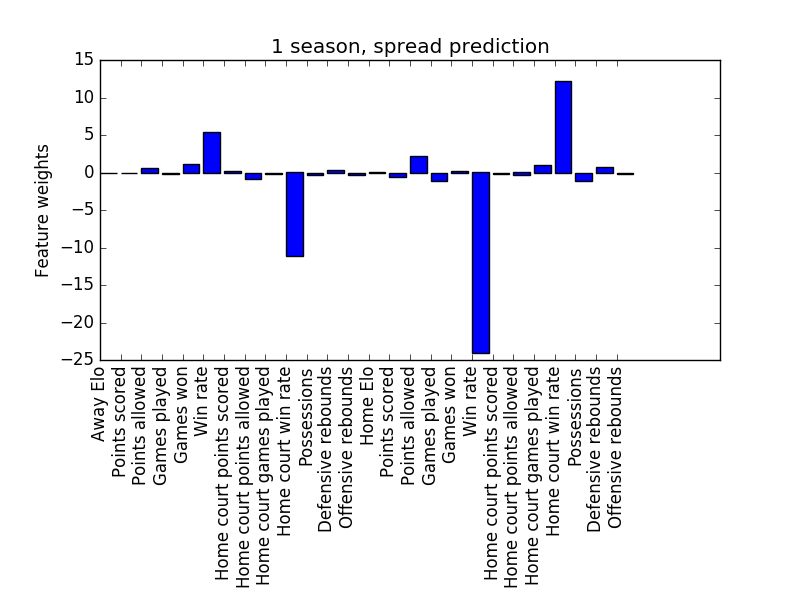
\includegraphics[width=1.2\linewidth]{code/figures/1season,spreads.png}
  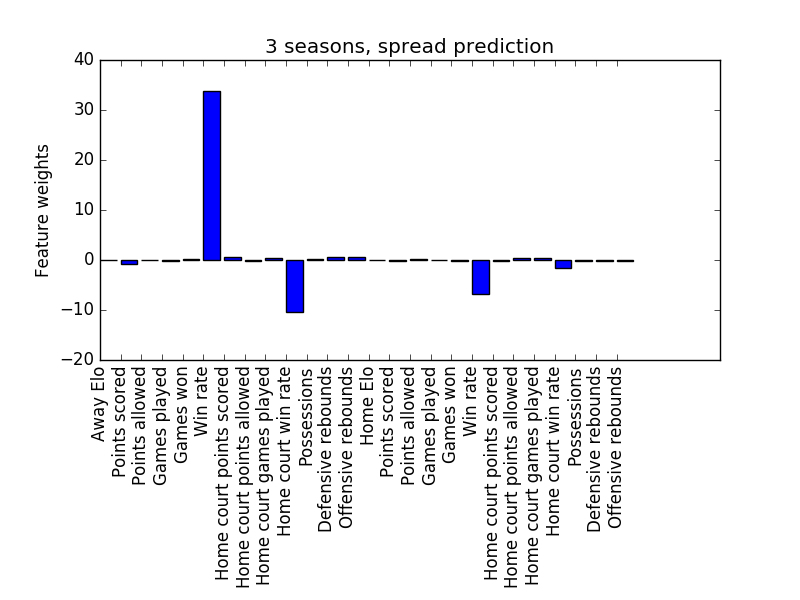
\includegraphics[width=1.2\linewidth]{code/figures/3seasons,spreads.png}
\end{multicols}
\caption{Linear classifier feature weights}
\end{figure}

Interestingly, when we train the linear classifier using only the win rate features, the classifier actually performs slightly better than with all the features. The numbers in Table 3 and 4 represent the accuracies and spread errors of the classifiers trained on all features and only win rate features when trained on one and three seasons of data, respectively. These findings seem to contradict the conclusions earlier in that adding more complex features such as home court advantage and rebounds improved the accuracy of the classifier. This could be due to overfitting to the number of features, especially in short periods of time in which averages might not necessarily be as representative of the overall skill level of a team.

\begin{table}
  \begin{center}
    \begin{tabular}{ | c | c | c | }
      \hline
                         & Win/Lose Accuracy & Spread Error  \\ \hline
      All features       & 66.9\%            & 13.6         \\ \hline
      Only win rate      & 70.7\%            & 8.95         \\ \hline
    \end{tabular}
  \end{center}
  \caption{Classifier performance on 1 season}
\end{table}

\begin{table}
  \begin{center}
    \begin{tabular}{ | c | c | c | }
      \hline
                         & Win/Lose Accuracy & Spread Error  \\ \hline
      All features       & 68.6\%            & 9.29         \\ \hline
      Only win rate      & 68.7\%            & 9.14         \\ \hline
    \end{tabular}
  \end{center}
  \caption{Classifier performance on 3 seasons}
\end{table}




\section{Evaluation}
In addition to calculating and analyzing the average spread error, we also compared our spreads predictions against other betting authorities' spreads. After creating a scaper which scraped the spreads posted by other betting authorities, we were able to determine the rate at which our spread would have beaten the betting authority's spread. This would occur in two scenarios: (1) if our predicted spread indicates that the winning team would have won by more than the other betting authority's predicted spread (e.g. if our spread is -8 and the other betting authority's spread is -5 on a game in which the favored team won by more than five points), or (2) if the predicted spread indicates that the winning team would have won by less or lost compared with theo ther begging authority's predicted spread (e.g. if our spread is +2 and the other betting authority's spread is -5 on a game in which the favored team lost or won by less than five points).


\section{Potential sources of failure}
Some drawbacks to the algorithm presented here include the fact that we do not examine individual player data. This was a choice made largely due to the fact that individualized player data is quite difficult to obtain, especially in quantities large enough for accurate training, validation, and testing. Because we look at a team's performance overall so far in the season however, this means that our algorithm is susceptible to changes in starting player lineups, player trades made during the season, and player injuries. Thus, despite the acceptable performance of our algorithm, we do identify this source of weakness in the ability to predict spreads and classify win/loss in matchups. Future iterations of the algorithm would therefore primarily seek to address these potential sources of failure in order to further improve and refine the overall predictive power of the algorithm.


\section{Breakdown of individual work}
The breakdown of work between the two members of the group largely followed that given in the original project proposal. Andrea and Tyson jointly worked on preliminary review of the current techniques and the state of the art. Following this, Tyson was primarily involved in the collection of game data from past seasons, and Andrea created the scraper to collect data on historical spreads put out by various betting organizations on previous games. Andrea explored preliminary models such as linear regression, logistic regression, and regression with various basis functions and various degrees of regularization, and Tyson chiefly explored a neural network approach. As discussed during the project proposal meeting, we decided not to implement a convolutional neural network for this problem, as the architecture did not fit the structure of the problem as closely. We each tested the models we worked on against data test sets and historical spreads, and we split the writing up of the report equally.


\end{document}


% This document was modified from the file originally made available by
% Pat Langley and Andrea Danyluk for ICML-2K. This version was
% created by Lise Getoor and Tobias Scheffer, it was slightly modified
% from the 2010 version by Thorsten Joachims & Johannes Fuernkranz,
% slightly modified from the 2009 version by Kiri Wagstaff and
% Sam Roweis's 2008 version, which is slightly modified from
% Prasad Tadepalli's 2007 version which is a lightly
% changed version of the previous year's version by Andrew Moore,
% which was in turn edited from those of Kristian Kersting and
% Codrina Lauth. Alex Smola contributed to the algorithmic style files.
